\documentclass[]{report}
\usepackage{amsmath,amsfonts}
\usepackage{graphicx}
\usepackage{url}
\usepackage[hidelinks]{hyperref}
\usepackage{tikz}
\usetikzlibrary{arrows.meta, decorations.pathreplacing, decorations.pathmorphing}

% Title Page
\title{{\huge  TITLE} \\
{\small Automatic Control\\
Electronic Engineering for Intelligent Vehicles\\
University of Bologna\\
A.A. 202X-202X}}
\author{Student A and Student B and ...}


\begin{document}
\maketitle

\begin{abstract}
	Here briefly detail  the aims of the project.
\end{abstract}

\chapter{Introduction}
\section{Motivations}
Explain why the selected application is important. Describe the application with informal words.

\section{Contributions}
Describe what this project deals with. What has been done to solve the problem presented in the motivations.

\section{State of art and literature comparison}
List the closest works that deal with the same problem and compare the achievement obtained and the strategies exploited in this paper. For the search of the literature use \url{https://ieeexplore.ieee.org/Xplore/home.jsp} and \url{https://www.sciencedirect.com/}.

\section{Organisation of the manuscript}
Describe what the reader finds in each of the Sections of this manuscript.

\section{List of the symbols}
Here list all the symbols used in the manuscript and add a description to each of them (Use the International System of Units \url{https://en.wikipedia.org/wiki/International_System_of_Units}).

\chapter{MAIN BODY}
Change the title with the name of the selected application

\section{Model and Problem Formulation}
In this section, we formulate the control problem for the active suspension system of a half-car model. This system aims to regulate both the vertical position and the perceived pitch angle of the vehicle body, enhancing ride comfort and handling. The model is described by a nonlinear dynamic system influenced by road disturbances, actuator forces, and sensor measurements.

The general form of the system is expressed as:
\begin{align}
	\dot{x} &= f(x, u, w) \\
	y &= h(x, u, w) \\
	e &= h_e(x, u, w)
\end{align}

Where:
\begin{itemize}
	\item $x \in \mathbb{R}^n$ is the \textbf{state vector},
	\item $u \in \mathbb{R}^p$ is the \textbf{control input vector},
	\item $y \in \mathbb{R}^q$ is the \textbf{measured output vector},
	\item $e \in \mathbb{R}^{l_m}$ is the \textbf{control error (goal)},
	\item $d \in \mathbb{R}^{l_d}$ is the \textbf{disturbance vector},
	\item $r \in \mathbb{R}^{l_r}$ is the \textbf{reference signal},
	\item $\nu \in \mathbb{R}^q$ is the \textbf{sensor noise},
	\item $w = \text{col}(d, \nu, r)$ is the \textbf{exogenous input}.
\end{itemize}
\begin{equation}
	\label{eq:FormulaA}
	\begin{aligned}
		\dot{x} &= f(x,u) && x(t_0) = x_0
\\
y &= h(x,u)
\end{aligned}
\end{equation}
\subsection*{Assumptions}

To make the problem tractable and to ensure solvability of the control task, we impose the following assumptions:

\begin{enumerate}
	\item The exogenous input $w$ is not directly measurable.
	\item Disturbances $d$ are bounded.
	\item Reference signal $r$ and its first derivatives are known.
	\item Bounded disturbances imply bounded internal states and outputs.
	\item The system has at least as many control inputs as control goals, i.e., $p \geq l_m$.
	\item The control error $e$ can be reconstructed from the output $y$: $\exists E$ such that $e = E(y)$.
\end{enumerate}

These assumptions lay the theoretical foundation required to design a control law capable of driving the error $e$ to zero despite the presence of unknown disturbances and sensor noise.

\section{Model Analysis}
\subsection{Dynamic Model}

The state vector describes the dynamic behavior of the half-car model, capturing both translational and rotational motion of the vehicle body as well as road-induced pitch disturbances at the front and rear axles. The state vector consists of eight components and is expressed as follows:
\begin{align}
	x = \begin{bmatrix}
		x_1 \\ x_2 \\ x_3 \\ x_4 \\ x_5 \\ x_6 \\ x_7 \\ x_8
	\end{bmatrix} =
	\begin{bmatrix}
		z - z_g \\
		\dot{z} - \dot{z}_g \\
		\theta \\
		\dot{\theta} \\
		\theta_{gf} \\
		\omega_{gf} \\
		\theta_{gr} \\
		\omega_{gr}
	\end{bmatrix}
\end{align}

Here:
\begin{itemize}
	\item $z$ is the vertical displacement of the vehicle’s center of mass (CoM), and $z_g$ is the vertical displacement of the road surface.
	\item $\dot{z}$ and $\dot{z}_g$ are the vertical velocities of the vehicle body and road, respectively.
	\item $\theta$ is the pitch angle of the vehicle body, and $\dot{\theta}$ its angular velocity.
	\item $\theta_{gf}$ and $\omega_{gf}$ are the road pitch angle and its rate of change at the front axle.
	\item $\theta_{gr}$ and $\omega_{gr}$ are the corresponding quantities at the rear axle.
\end{itemize}

This formulation enables the model to capture the full set of dynamics necessary for accurate representation of vehicle behavior under road disturbances and control inputs.

\begin{center}
	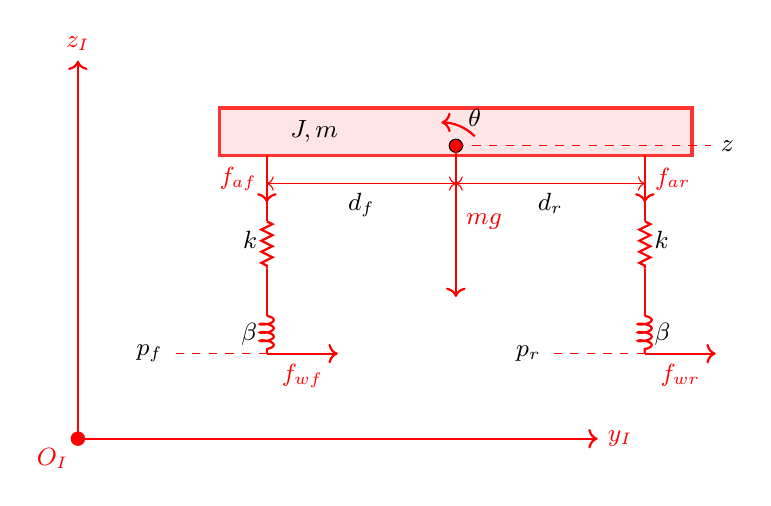
\begin{tikzpicture}[scale=1.2, every node/.style={font=\small}]
		
		% Coordinate axes
		\draw[->, thick, red] (-3.5,-1.5) -- (-3.5,2.5) node[above] {$z_I$};
		\draw[->, thick, red] (-3.5,-1.5) -- (2,-1.5) node[right] {$y_I$};
		\filldraw[red] (-3.5,-1.5) circle (2pt) node[below left] {$O_I$};
		
		% Sprung mass (body)
		\filldraw[color=red!80, fill=red!10, very thick] (-2,1.5) rectangle (3,2);
		\node at (-1,1.75) {$J, m$};
		
		% Center of mass
		\draw[fill=red] (0.5,1.6) circle (0.07);
		\draw[->, thick, red] (0.5,1.6) -- (0.5,0) node[midway,right] {$mg$};
		
		% pitch angle psi
		\draw[->, red, thick] (0,1.5) ++(0.7,0.2) arc[start angle=45,end angle=90,radius=0.5];
		\node at (0.7,1.9) {$\theta$};
		
		% Front suspension
		\draw[thick, red] (-1.5,1.5) -- (-1.5,0.8);
		\draw[thick, red, decorate, decoration={zigzag,segment length=4,amplitude=2}] (-1.5,0.8) -- (-1.5,0.3);
		\draw[thick, red] (-1.5,0.3) -- (-1.5,-0.2);
		\node[left] at (-1.5,0.6) {$k$};
		\draw[thick, red, decorate, decoration={coil,aspect=0.3, segment length=3}] (-1.5,-0.2) -- (-1.5,-0.6);
		\node[left] at (-1.5,-0.4) {$\beta$};
		\draw[->, thick, red] (-1.5,1.5) -- (-1.5,1.0) node[midway,left] {$f_{af}$};
		
		% Rear suspension
		\draw[thick, red] (2.5,1.5) -- (2.5,0.8);
		\draw[thick, red, decorate, decoration={zigzag,segment length=4,amplitude=2}] (2.5,0.8) -- (2.5,0.3);
		\draw[thick, red] (2.5,0.3) -- (2.5,-0.2);
		\node[right] at (2.5,0.6) {$k$};
		\draw[thick, red, decorate, decoration={coil,aspect=0.3, segment length=3}] (2.5,-0.2) -- (2.5,-0.6);
		\node[right] at (2.5,-0.4) {$\beta$};
		\draw[->, thick, red] (2.5,1.5) -- (2.5,1.0) node[midway,right] {$f_{ar}$};
		
		% Front and rear wheel forces
		\draw[->, thick, red] (-1.5,-0.6) -- (-0.75,-0.6) node[midway,below] {$f_{wf}$};
		\draw[->, thick, red] (2.5,-0.6) -- (3.25,-0.6) node[midway,below] {$f_{wr}$};
		
		% Ground heights
		\draw[dashed, red] (-1.5,-0.6) -- (-2.5,-0.6);
		\node[left] at (-2.5,-0.6) {$p_f$};
		\draw[dashed, red] (2.5,-0.6) -- (1.5,-0.6);
		\node[left] at (1.5,-0.6) {$p_r$};
		
		% Distances df and dr
		\draw[<->, red] (0.5,1.2) -- (-1.5,1.2);
		\node[below] at (-0.5,1.2) {$d_f$};
		\draw[<->, red] (0.5,1.2) -- (2.5,1.2);
		\node[below] at (1.5,1.2) {$d_r$};
		
		% Labels z
		\draw[dashed, red] (0.5,1.6) -- (3.2,1.6);
		\node[right] at (3.2,1.6) {$z$};
		
	\end{tikzpicture}
\end{center}

The suspension system in the half-car model is influenced by two actuators—one at the front and one at the rear. These actuators generate forces that contribute to both the vertical and rotational dynamics of the vehicle body. The control input vector is defined as:


\begin{align}
	u = \begin{bmatrix}
		u_1 \\
		u_2
	\end{bmatrix} =
	\begin{bmatrix}
		f_{af} + f_{ar} \\
		f_{af} d_f - f_{ar} d_r
	\end{bmatrix}
\end{align}

In this expression, $f_{af}$ and $f_{ar}$ are the forces generated by the front and rear suspension actuators, respectively. The parameters $d_f$ and $d_r$ denote the distances from the vehicle's center of mass to the front and rear axles. The first control input, $u_1$, represents the total vertical force acting on the vehicle body due to both actuators. The second input, $u_2$, represents the net moment about the vehicle’s center of mass generated by these forces, which directly influences the pitch motion.


The evolution of the system over time is governed by a set of first-order differential equations derived from Newton’s laws for both translational and rotational motion. The dynamic model is expressed as:

\begin{align}
	\dot{x} = \begin{bmatrix}
		x_2 \\
		f_2 - \ddot{z}_g \\
		x_4 \\
		f_4 \\
		x_6 \\
		\alpha_{gf} \\
		x_8 \\
		\alpha_{gr}
	\end{bmatrix}
\end{align}

Where:
\begin{itemize}
	\item $f_2$ is the net vertical acceleration of the vehicle body due to suspension forces, gravity, and actuator inputs.
	\item $f_4$ is the pitch angular acceleration about the vehicle’s center of mass.
	\item $\ddot{z}_g$ is the vertical acceleration of the road surface.
	\item $\alpha_{gf}$ and $\alpha_{gr}$ are the angular accelerations of the road surface at the front and rear axles, respectively.
\end{itemize}

These dynamics describe how the vehicle responds to both internal control actions and external disturbances, including variations in road pitch encountered at different points along the vehicle chassis.

In this representation, $f_2$ is given by:

\begin{align}
	f_2 &= -g + \frac{1}{m}(f_{sf} + f_{sr}) + \frac{u_1}{m} \\
\end{align}

The pitch angular acceleration $f_4$ is given by:

\begin{align}	
	f_4 &= \frac{1}{J}(f_{sf} d_f - f_{sr} d_r + u_2 + f_{wf} l_{f} + f_{wr} l_{r})
\end{align}


The suspension deflections and velocities are:

\begin{align}
	s_1 &= x_1 + d_f(\sin x_3 - \sin x_5), \quad s_3 = x_1 - d_r(\sin x_3 - \sin x_5) \\
	s_2 &= x_2 + d_f(x_4 \cos x_3 - x_6 \cos x_5), \quad s_4 = x_2 - d_r(x_4 \cos x_3 - x_6 \cos x_5)
\end{align}

Suspension forces are modeled as spring-damper systems:

\begin{align}
	f_s(p, v) = -k p - \beta v
\end{align}

\subsection{Sensor Model}

The effectiveness of the control architecture relies heavily on the accurate and timely acquisition of physical quantities related to the vehicle's motion and posture. To this end, the half-car system is equipped with a set of onboard sensors, specifically selected to ensure observability of the dynamic model and to allow real-time feedback control.

\paragraph{Measurement Vector.}
The complete sensor output is gathered in the measurement vector:

\begin{align}
	y = \begin{bmatrix}
		y_y \\ y_z \\ y_g \\ y_l \\ y_r
	\end{bmatrix} =
	\begin{bmatrix}
		\sin x_3(f_2 + g) + \cos x_3(f_{wr} + f_{wf})/m \\
		\cos x_3(f_2 + g) - \sin x_3(f_{wr} + f_{wf})/m \\
		x_4 \\
		s_1 \\
		s_3
	\end{bmatrix} + \nu
\end{align}

This vector includes measurements from two accelerometers, one gyroscope, and two linear potentiometers, all subject to additive noise $\nu$.

\paragraph{Accelerometers.}
The first two components $y_y$ and $y_z$ represent the lateral and vertical accelerations measured in the vehicle’s body-fixed reference frame. These measurements are obtained via two MEMS accelerometers mounted at the vehicle's center of mass. Due to the non-inertial frame of reference, the accelerations are nonlinear combinations of translational and rotational dynamics and include the gravitational component projected along the vehicle's pitch angle $x_3 = \theta$.

These measurements are used to estimate the apparent pitch angle $\theta_a$, which is a key feedback signal for pitch stabilization control. We assume a typical sensor such as the \textbf{STMicroelectronics LIS3DH}, offering 12-bit resolution, low noise density ($\sim50~\mu g/\sqrt{Hz}$), and a digital output interface.

\paragraph{Gyroscope.}
The third component $y_g$ corresponds to the pitch angular rate $\dot{\theta}$, measured directly by a gyroscope mounted on the vehicle frame. This measurement provides high-frequency information essential for dynamic feedback control and stability monitoring.

A typical device used could be the \textbf{Bosch BMI160} inertial measurement unit (IMU), with integrated accelerometer and gyroscope, capable of delivering low-latency angular rate data with high sensitivity (16-bit ADC) and low drift. The sensor is assumed to be rigidly fixed to the main chassis near the center of rotation to minimize errors due to offset and vibration.

\paragraph{Suspension Potentiometers.}
The fourth and fifth entries $y_l$ and $y_r$ are deflection measurements of the front and rear suspension struts, modeled by the quantities $s_1$ and $s_3$. These values are acquired via linear position sensors (e.g., \textbf{Honeywell MLH Series}) mounted along the suspension path to detect extension or compression relative to the static rest position.

These readings give direct insight into the interaction between the vehicle and the road surface, reflecting terrain irregularities, road disturbances, and load shifts. Additionally, they are fundamental to compute control actions that regulate ride comfort and load distribution.

\paragraph{Noise Modeling.}
All sensor measurements are corrupted by additive noise:

\[
\nu = \begin{bmatrix}
	\nu_y & \nu_z & \nu_g & \nu_l & \nu_r
\end{bmatrix}^T
\]

We assume Gaussian-distributed noise with known standard deviations derived from the sensor datasheets. Noise in the accelerometers and gyroscope may include both white noise and low-frequency bias drift, while potentiometers may exhibit quantization and thermal noise. These uncertainties justify the implementation of robust filtering (e.g., Kalman filters) and noise-resilient control laws.

\paragraph{Sensor Placement and Observability.}
The sensor configuration is designed to ensure full observability of the system state vector $x$ required for control. The accelerometers and gyroscope reconstruct the translational and rotational dynamics, while the suspension sensors resolve wheel-body interactions. This sensor suite has been tested in simulation to confirm that it enables estimation of all states through standard observers.

\paragraph{Practical Considerations.}
While alternative sensors such as LIDAR, GPS, or magnetometers could enhance localization in other contexts, they are not considered here due to their inadequacy in indoor or suspension-focused scenarios. For example, GPS is unsuitable for fine-grained control of vertical dynamics or in indoor testing environments, and magnetometers are highly susceptible to interference from ferromagnetic chassis components and electromagnetic noise from motors.

The selected sensor set offers a balance between cost, precision, and real-time capability, making it well-suited for embedded automotive platforms focused on suspension control and ride dynamics.


\paragraph{Control Objectives.}

We define the apparent pitch angle $\theta_a$ using accelerometer data:

\begin{align}
	\theta_a = \sin^{-1} \left( \frac{y_y}{\sqrt{y_y^2 + y_z^2}} \right)
\end{align}

The control error vector is defined as:

\begin{align}
	e = \begin{bmatrix}
		\frac{y_f d_r + y_r d_f}{d_r + d_f} - r_z \\
		\theta_a - r_\theta
	\end{bmatrix}
\end{align}

This error describes deviations from the desired vertical height and perceived pitch. The control task is to design $u$ to drive $e \rightarrow 0$ in the presence of disturbances and noise.

The second component of the error vector $he(x,u,w)$ captures the deviation from a desired apparent pitch angle $\theta_a$, which reflects the passenger-perceived acceleration. It is defined through the nonlinear relationship:
\[
\sin(\theta_a) = \frac{y_y}{\sqrt{y_y^2 + y_z^2}} \quad \Rightarrow \quad \theta_a = \sin^{-1}\left(\frac{y_y}{\sqrt{y_y^2 + y_z^2}}\right),
\]
where $y_y$ and $y_z$ are the accelerometer outputs along the body-frame $y$ and $z$ axes, respectively. This formulation provides an estimate of the pitch experienced by passengers during acceleration, braking, or uneven ground contact.


The complete output error function thus becomes:
\[
he(x, u, w) =
\begin{bmatrix}
	\displaystyle \frac{(s_1 + \nu_f) d_r + (s_3 + \nu_r) d_f}{d_r + d_f} - r_z \\
	\displaystyle \sin^{-1}\left( \frac{h_1 + \nu_y}{\sqrt{(h_1 + \nu_y)^2 + (h_2 + \nu_z)^2}} \right) - r_\theta
\end{bmatrix},
\]
where $s_1$, $s_3$ are suspension deflections, $h_1$, $h_2$ are derived from dynamic equations, and $\nu_i$ are sensor noise terms. This formulation ensures the controller minimizes both height and perceptual pitch deviations.


\subsection{Linear Model Analysis}

To support the development of an effective suspension controller and gain insight into the vehicle's dynamic behavior, we examine a linearized model of a half-car system. This analysis is performed around a nominal equilibrium point, where the vehicle is at rest with zero pitch angle and no vertical or angular velocities. The focus is on the open-loop dynamics of the vehicle body, excluding actuator behavior and wheel compliance.

The model captures the essential vertical (heave) and angular (pitch) motions of the chassis. The state vector is defined as:

\[
x = \begin{bmatrix}
	z - z_0 \\
	\dot{z} \\
	\theta \\
	\dot{\theta}
\end{bmatrix}
\]

where \( z_0 \) is the vertical position of the center of mass at static equilibrium, and \( \theta \) denotes the pitch angle of the chassis. The state-space representation of the system is given by:

\[
\dot{x} = A_{\text{int}} x
\]

We are gonna analyze this reduced 4x4 matrix, ignoring the 4 exogenous states, the reason behind this is explained later in the Reachability chapter.\textbf{INCLUDI NUMERO CAPITOLO}  All parameters used to find the numeric matrixes are based on the Tesla Model S, a car suitable for this type of active suspensions and with same suspension paramethers on front and rear axle, this simplifies slighlty our model:
\[
A_{\text{int}} =
\begin{bmatrix}
	0 & 1 & 0 & 0 \\
	-55.2995 & -3.68664 & 6.52535 & 0.435023 \\
	0 & 0 & 0 & 1 \\
	1.4538 & 0.0969199 & -27.158 & -1.81053 
\end{bmatrix}
\]

This matrix characterizes the coupled dynamics of the system, with off-diagonal elements indicating interaction between vertical and angular motions. Such coupling arises naturally in a physical half-car system, where vertical displacements can induce pitching, and vice versa.

\subsubsection{Open-Loop Dynamics}

To evaluate the system's stability and transient behavior, we compute the eigenvalues of the matrix \( A_{\text{int}} \) by solving the characteristic equation:

\[
\det(A_{\text{int}} - \lambda I) = 0
\]

The resulting eigenvalues are:

\[
\lambda_{1,2} = -1.55 \pm j6.28, \quad \lambda_{3,4} = -2.47 \pm j5.10
\]

These eigenvalues form two complex-conjugate pairs, each with negative real parts. This indicates that the system is asymptotically stable in open loop. The imaginary components represent oscillatory behavior in the system's response to disturbances.

\begin{itemize}
	\item The eigenvalues \( \lambda_{1,2} \) correspond to a lightly damped oscillatory mode with a higher frequency.
	\item The eigenvalues \( \lambda_{3,4} \) correspond to a more heavily damped mode with a lower oscillation frequency.
\end{itemize}

Due to the coupling present in \( A_{\text{int}} \), these modes represent mixed heave-pitch dynamics rather than purely vertical or angular motions. This hybrid behavior implies that any disturbance in one degree of freedom can propagate to the other, necessitating a control strategy that accounts for this interaction.

The system’s open-loop stability ensures that disturbances decay over time, but the oscillatory nature of the transients may degrade ride comfort and vehicle handling. Therefore, active suspension control is warranted to suppress these vibrations more rapidly, reduce settling time, and improve overall vehicle performance.

In summary, the linearized model described by \( A_{\text{int}} \) reveals a stable but dynamically coupled system with oscillatory characteristics. These insights are essential for the design of coordinated control strategies that enhance both ride quality and dynamic response.



\newpage
\section{Control}

\subsubsection{Reachability}




In this section, a reachability analysis is carried out to determine which parts of the system's state space can be influenced by the control input. Starting from the linearized state-space system:

\[
\dot{\tilde{x}} = A \tilde{x} + B_1 \tilde{u}
\]

we aim to identify which states can be driven from the origin to a desired position through the control input $\tilde{u}$. The reachability matrix is defined as:

\[
\mathcal{R} = \left[ B_1 \quad AB_1 \quad A^2B_1 \quad \dots \quad A^{n-1}B_1 \right]
\]

A linear time-invariant system is said to be \textbf{fully reachable} (or controllable from the origin) if the rank of $\mathcal{R}$ is equal to $n$, the number of state variables. In such a case, it is possible to design a state feedback controller that places all eigenvalues of the closed-loop system arbitrarily.


In our case, the system has $n = 8$ state variables. These include both the vehicle body dynamics (vertical position and velocity, pitch angle and rate) and road-related exogenous components (front and rear road pitch angles and their derivatives). The control input $\tilde{u} \in \mathbb{R}^2$ acts through actuators located at the front and rear suspensions, influencing primarily the body dynamics of the vehicle.

However, the states related to the road excitation are not directly controllable. As such, only a subset of the full state vector can be affected by $\tilde{u}$. Upon computation of the reachability matrix $\mathcal{R}$ using the specific system matrices $A$ and $B_1$, we obtain:


\[
A =
\begin{bmatrix}
	0 & 1 & 0 & 0 & 0 & 0 & 0 & 0 \\
	-55.2995 & -3.68664 & 6.52535 & 0.435023 & 37.659 & -44.1843 & 2.5106 & -2.94562 \\
	0 & 0 & 0 & 1 & 0 & 0 & 0 & 0 \\
	1.4538 & 0.0969199 & -27.158 & -1.81053 & 11.4274 & 15.7306 & 0.761825 & 1.04871 \\
	0 & 0 & 0 & 0 & 1 & 0 & 0 & 0 \\
	0 & 0 & 0 & 0 & 0 & 1 & 0 & 0 \\
	0 & 0 & 0 & 0 & 0 & 0 & 0 & 0 \\
	0 & 0 & 0 & 0 & 0 & 0 & 0 & 0 
\end{bmatrix}
\]

\[
B_1 =
\begin{bmatrix}
	0 & 0 \\
	0.000921659 & 0  \\
	0 & 0 \\
	0 & 0.000205339 \\
	0 & 0 \\
	0 & 0 \\
	0 & 0 \\
	0 & 0 \\
	
\end{bmatrix}
\]


\begin{verbatim}
R = ctrb(A, B1);
rank_R = rank(R);

\end{verbatim}

\[
\text{rank}(\mathcal{R}) = 4 < 8
\]

This indicates that the system is \textbf{not fully reachable}. Only the four states corresponding to the internal dynamics of the vehicle body are reachable, while the remaining four states — associated with the road profile — are uncontrollable and must be treated as external disturbances. Consequently, control strategies such as state feedback and optimal control (e.g., LQR) can only be designed for the reachable subspace.

\paragraph{Reduced Reachability Analysis}

In the present model, the state vector $\tilde{x} \in \mathbb{R}^8$ includes eight components. However, the last four states represent environmental or road-related variables (e.g., road profile curvature), which evolve independently of the control input $\tilde{u}$. These are known as \textbf{exogenous states} and are not directly controllable.

Therefore, we perform reachability analysis only on the first four states, which represent the internal vehicle dynamics and are influenced by control inputs. Let $A_{\text{int}}$ and $B_{1, \text{int}}$ be the upper-left $4 \times 4$ and $4 \times 2$ blocks of matrices $A$ and $B_1$:

\[
A_{\text{int}} =
\begin{bmatrix}
	0 & 1 & 0 & 0 \\
	-55.2995 & -3.68664 & 6.52535 & 0.435023 \\
	0 & 0 & 0 & 1 \\
	1.4538 & 0.0969199 & -27.158 & -1.81053 
\end{bmatrix}
\]

\[
B_{1,\text{int}} =
\begin{bmatrix}
	0 & 0 \\
	0.000921659 & 0  \\
	0 & 0 \\
	0 & 0.000205339 

\end{bmatrix}
\]

\[
\dot{\tilde{x}}_{\text{int}} = A_{\text{int}} \tilde{x}_{\text{int}} + B_{1,\text{int}} \tilde{u}
\]

The reachability matrix becomes:

\[
\mathcal{R}_{\text{int}} = \left[ B_{1,\text{int}} \quad A_{\text{int}}B_{1,\text{int}} \quad A_{\text{int}}^2B_{1,\text{int}} \quad A_{\text{int}}^3B_{1,\text{int}} \right]
\]

We then evaluate the rank of this matrix using MATLAB's \texttt{ctrb} function:

\begin{verbatim}
	R_int = ctrb(A_int, B1_int);
	rank(R_int)
\end{verbatim}

The resulting rank is 4, which confirms that the internal subsystem is fully reachable.

\paragraph{Stabilizability and the Hurwitz Condition}

According to control theory, if the system is fully reachable, it is possible to design a state feedback control law:

\[
\tilde{u} = K_S \tilde{x}_{\text{int}}
\]

such that the closed-loop matrix:

\[
A_{\text{int}} + B_{1,\text{int}} K_S
\]

is \textbf{Hurwitz}, meaning that all of its eigenvalues lie in the left half of the complex plane. This ensures that the closed-loop system is \textbf{BIBS stable} (Bounded Input Bounded State): all state trajectories remain bounded in response to bounded inputs.

In conclusion, while the full model is not entirely reachable due to the presence of exogenous states, the subsystem representing the vehicle dynamics is fully reachable and can be stabilized using linear state feedback.


\subsubsection{Integral Action}

While the stabilizer matrix $K_S$ ensures the stability of the internal system under feedback control, an integral action is required to eliminate steady-state error in the presence of unknown constant disturbances $\tilde{w}$.

The regulated error $\tilde{e}$ is defined as:
\[
\tilde{e} = C_e \tilde{x} + D_{1e} \tilde{u} + D_{2e} \tilde{w}
\]

To implement integral control, we introduce a new integral state $\eta$:
\[
\dot{\eta} = \tilde{e}
\]

This leads to an extended state vector:
\[
x_e = \begin{bmatrix} \tilde{x} \\ \eta \end{bmatrix}
\]

The extended system dynamics are:
\[
\dot{x}_e = \bar{A} x_e + \bar{B}_1 \tilde{u} + \bar{B}_2 \tilde{w}
\]
where
\[
\bar{A} = \begin{bmatrix}
	A & 0 \\
	C_e & 0
\end{bmatrix},
\quad
\bar{B}_1 = \begin{bmatrix}
	B_1 \\
	D_{1e}
\end{bmatrix},
\quad
\bar{B}_2 = \begin{bmatrix}
	B_2 \\
	D_{2e}
\end{bmatrix}
\]

To verify whether the extended system is controllable (reachable), we compute the reachability matrix:
\[
\mathcal{R}_e = \left[\bar{B}_1 \quad \bar{A}\bar{B}_1 \quad \bar{A}^2\bar{B}_1 \quad \cdots \quad \bar{A}^{n+q-1} \bar{B}_1 \right]
\]

where $n$ is the number of original state variables and $q$ is the number of integrator states. In our model, $n=4$ (excluding the two uncontrollable states) and $q=2$, so we expect:
\[
\text{rank}(\mathcal{R}_e) = 6
\]

The reachability matrix is constructed in MATLAB using:

\begin{verbatim}
	Ae = [A, zeros(6,2); Ce, zeros(2,2)];
	B1e = [B1; D1e];
	Re = ctrb(Ae, B1e);
	rank(Re)
\end{verbatim}

\textbf{Result:}  
The output of the command confirms that $\text{rank}(\mathcal{R}_e) = 6$, i.e., the extended system is fully reachable.

\textbf{Conclusion:}  
Since the extended system is reachable, it is possible to design a state feedback control law of the form:
\[
\tilde{u} = \bar{K} x_e = K_S \tilde{x} + K_I \eta
\]
such that the closed-loop matrix $\bar{A} + \bar{B}_1 \bar{K}$ is Hurwitz. This guarantees asymptotic stability of the augmented system and drives the regulation error $\tilde{e}$ to zero.



\subsubsection{Observability}

Up to this point, the system state $\tilde{x}$ has been assumed to be known. However, this assumption is often unrealistic, particularly when some state variables are not directly measurable. For this reason, a state observer is required to estimate the internal states based on measurable outputs.

Given that the last four states of $\tilde{x}$ are exogenous and not influenced by the system dynamics, we restrict our observability analysis to the internal dynamics only, i.e., $\tilde{x}_{\text{int}} \in \mathbb{R}^4$.

Let $C_{\text{int}}$ be the output matrix corresponding to the internal states. Then, the observability matrix is given by:

\[
\mathcal{O} = \begin{bmatrix}
	C_{\text{int}} \\
	C_{\text{int}} A_{\text{int}} \\
	C_{\text{int}} A_{\text{int}}^2 \\
	C_{\text{int}} A_{\text{int}}^3 \\
\end{bmatrix}
\]

\[
C_{\text{int}} =
\begin{bmatrix}
	0 & 0 & 9.81 & 0 \\
	-55.2995 & -3.68664 & 6.52535 & 0.435023 \\
	0 & 0 & 0 & 1 \\
	1 & 0 & 1.362 & 0  \\
	1 & 0 & -1.598 & 0 \\
	0 & 0 & 0 & 0 \\
	0 & 0 & 0 & 0 
\end{bmatrix}
\]

Using MATLAB, we compute:

\begin{verbatim}
	O = obsv(A_int, C_int);
	rank(O)
\end{verbatim}

If $\text{rank}(\mathcal{O}) = n = 4$, the system is \textbf{fully observable}, and it is possible to construct a full-order Luenberger observer:
\textbf{DA CAMBIARE CON FORMULA KALMAN FILTER?}
\[
\dot{\hat{x}}_{\text{int}} = A_{\text{int}} \hat{x}_{\text{int}} + B_{1,\text{int}} \tilde{u} + K_O(y - C_{\text{int}} \hat{x}_{\text{int}})
\]

where $K_O$ is the observer gain. By properly choosing $K_O$, the eigenvalues of $(A_{\text{int}} - K_O C_{\text{int}})$ can be placed in the left half-plane to make the observer error dynamics stable. That is, the matrix must be \textbf{Hurwitz} to ensure convergence of the estimate $\hat{x}_{\text{int}}$ to the true internal state $\tilde{x}_{\text{int}}$.

We check observability with MATLAB:

\begin{verbatim}
	O = obsv(A_int, C_int);
	rank(O)
\end{verbatim}

\textbf{Conclusion:}  
The MATLAB analysis confirms that $\text{rank}(\mathcal{O}) = 4$, which equals the number of internal states. Therefore, the pair $(A_{\text{int}}, C_{\text{int}})$ is \textbf{fully observable}. This implies that there exists a matrix $K_O$ such that the observer error dynamics matrix $A_{\text{int}} - K_O C_{\text{int}}$ is \textbf{Hurwitz}.


This observability ensures that despite partial measurements, the entire controllable state can be reconstructed and regulated accordingly.




\chapter{Application}

\section{Simulator description}
\begin{center}
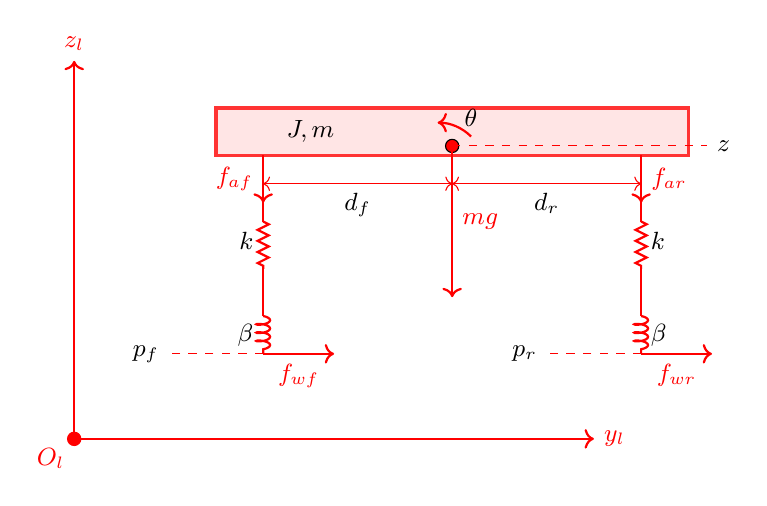
\begin{tikzpicture}[scale=1.2, every node/.style={font=\small}]
	
	% Coordinate axes
	\draw[->, thick, red] (-3.5,-1.5) -- (-3.5,2.5) node[above] {$z_l$};
	\draw[->, thick, red] (-3.5,-1.5) -- (2,-1.5) node[right] {$y_l$};
	\filldraw[red] (-3.5,-1.5) circle (2pt) node[below left] {$O_l$};
	
	% Sprung mass (body)
	\filldraw[color=red!80, fill=red!10, very thick] (-2,1.5) rectangle (3,2);
	\node at (-1,1.75) {$J, m$};
	
	% Center of mass
	\draw[fill=red] (0.5,1.6) circle (0.07);
	\draw[->, thick, red] (0.5,1.6) -- (0.5,0) node[midway,right] {$mg$};
	
	% pitch angle psi
	\draw[->, red, thick] (0,1.5) ++(0.7,0.2) arc[start angle=45,end angle=90,radius=0.5];
	\node at (0.7,1.9) {$\theta$};
	
	% Front suspension
	\draw[thick, red] (-1.5,1.5) -- (-1.5,0.8);
	\draw[thick, red, decorate, decoration={zigzag,segment length=4,amplitude=2}] (-1.5,0.8) -- (-1.5,0.3);
	\draw[thick, red] (-1.5,0.3) -- (-1.5,-0.2);
	\node[left] at (-1.5,0.6) {$k$};
	\draw[thick, red, decorate, decoration={coil,aspect=0.3, segment length=3}] (-1.5,-0.2) -- (-1.5,-0.6);
	\node[left] at (-1.5,-0.4) {$\beta$};
	\draw[->, thick, red] (-1.5,1.5) -- (-1.5,1.0) node[midway,left] {$f_{af}$};
	
	% Rear suspension
	\draw[thick, red] (2.5,1.5) -- (2.5,0.8);
	\draw[thick, red, decorate, decoration={zigzag,segment length=4,amplitude=2}] (2.5,0.8) -- (2.5,0.3);
	\draw[thick, red] (2.5,0.3) -- (2.5,-0.2);
	\node[right] at (2.5,0.6) {$k$};
	\draw[thick, red, decorate, decoration={coil,aspect=0.3, segment length=3}] (2.5,-0.2) -- (2.5,-0.6);
	\node[right] at (2.5,-0.4) {$\beta$};
	\draw[->, thick, red] (2.5,1.5) -- (2.5,1.0) node[midway,right] {$f_{ar}$};
	
	% Front and rear wheel forces
	\draw[->, thick, red] (-1.5,-0.6) -- (-0.75,-0.6) node[midway,below] {$f_{wf}$};
	\draw[->, thick, red] (2.5,-0.6) -- (3.25,-0.6) node[midway,below] {$f_{wr}$};
	
	% Ground heights
	\draw[dashed, red] (-1.5,-0.6) -- (-2.5,-0.6);
	\node[left] at (-2.5,-0.6) {$p_f$};
	\draw[dashed, red] (2.5,-0.6) -- (1.5,-0.6);
	\node[left] at (1.5,-0.6) {$p_r$};
	
	% Distances df and dr
	\draw[<->, red] (0.5,1.2) -- (-1.5,1.2);
	\node[below] at (-0.5,1.2) {$d_f$};
	\draw[<->, red] (0.5,1.2) -- (2.5,1.2);
	\node[below] at (1.5,1.2) {$d_r$};
	
	% Labels z
	\draw[dashed, red] (0.5,1.6) -- (3.2,1.6);
	\node[right] at (3.2,1.6) {$z$};
	
\end{tikzpicture}
\end{center}
Copy and past the Simulink block scheme and describe what each block does. Describe the set-up MATLAB file, where and how to change the parameters of the simulations. Remember to include also the sensor noises and realistic external disturbances.

\section{Simulation results}
Describe the simulation scenario: initial conditions, purpose of the simulation. Describe the results: are the results coherent with the expectation? If not why? Investigate the tuning: how the performance are affected by the selection of the parameters at disposal of the designer?

\chapter{Conclusions and further investigation}
Recap the main results obtained in the project and highlight eventual further investigation directions alogn which the performance could be improved. 

\newpage
\chapter*{Bibliography}
List the papers/books cited.

\newpage
\appendix
\chapter*{Appendix}
Use appendices to add technical parts which are instrumental for the completeness of the manuscript but are too heavy to be included inside the main text. Basically, appendices are exploited to let the main text cleaner and smoother. As example, the complete MATLAB listings can be reported in appendix.\\

HO

\end{document}          
